\documentclass[]{article}
\usepackage[koi8-r]{inputenc}
\usepackage{geometry}
\usepackage[pdftex]{graphicx}
\usepackage{wrapfig}
\graphicspath{{../images/}}
\DeclareGraphicsExtensions{.png}
%opening
\title{Astrometric Observations of the Main Uranian Satellites in the Pulkovo Observatory in 2007 -- 2016}
\author{Ershova A. P., Roschina E. A., Izmailov I. S., Khovrichev M. Yu.}
\geometry{left=2.5cm}
\geometry{right=2.5cm}
\geometry{top=2cm}
\geometry{bottom=2cm}
\begin{document}

\maketitle

\begin{abstract}
The results of observations of uranian satellites obtained with the Pulkovo Observatory 26-inch refractor in 2007 -- 2016 were presented. Almost 7000 CCD frames were analysed. The UCAC4 catalogue was used as an astrometric calibrator. Coordinates of Uranus were determined indirectly with the satellites? positions and their ephemeris relative to the planet. The O-C differences were calculated for each object using the INPOP13c planetary theory and Lainey's theory of the satellites motion. The mean values of the standard errors of (O?C) are within $0.02$ to $0.07$ arcsec. O-C absolute values are less than 0.05 arcsec. It is in a good agreement with ephemeris.
\end{abstract}

\section{Introduction}
High-precision theories of motion of the major planets and their satellites are necessary for researches of the Solar System formation and evolution, and for providing the ephemeridae for the future space missions. Construction of the theories requires an extensive observational material (Emelyanov, 2009).\par

In the twentieth century photographic observations of Uranus were performed at the Pulkovo Observatory (Kiseleva, Khrutskaya, 2007). Coordinates of the planet were determined with respect to the reference stars directly, uranian satellites were inaccessible for the photographic method\par

CCD-observations of Uranus have been started in 2007. The CCD-images of four main uranian satellites (Ariel, Umbriel, Titania and Oberon) are available for approximation. Final astrometric accuracy of the satellites? observations is similar to the positional precision presented in several recent investigations (Camargo et al., 2015, Khovrichev, 2009).  The fifth main satellite of Uranus (Miranda (u5)) is usually located within small angular distant from the planet (within bright part of scattered-light halo caused by Uranus). Therefore its images could not be correctly approximated.\par

The first results of observations of uranian satellites with CCD-camera and 26-inch refractor in Pulkovo were published in 2013. (Roschina et al., 2013). Published observations covered the period  2007 -- 2011. UCAC2 (Zacharias et al., 2010) was used as a reference catalog. Volume of observational data in current paper is significantly bigger. The resulted data sample contains satellites? position taken from August 2007 to Janiary 2016. The astrometric calibrations were performed with UCAC4 (Zacharias et al., 2013). This catalog provides significantly more stars in the field of view than UCAC2. It allows us to reach improvement of accuracy.

\section{Observations and mesaurements}
Current observations of Uranus are performing at the Pulkovo from the end of August to the begining of Janiary using the 26-inch refractor. The telescope is located at $59^o46' 15''$ north latitude, $30^o19'23''$ east longitude, altitude above the sea level is about 85 m. Aperture diameter of the telescope is 65 cm, focal length is 1041.3 cm, focal plane scale is 19''.80/mm in the center of image. The CCD camera FLI Pro Line 09000 is used. Size of the CCD matrix is 3056x3056 px, each of 12 $\mu$m. The field of view is $12'$x$12'$, the scale on the CCD frames is $0''.24$/px.\par
We obtained one normal place of each satellite available for observations in a night. Normal places were calculated on a basis of five independent measurements of individual positions. In turn we used a number of CCD frames combined together for each of these measurements. Observations were carried out by series: September 30, 2007 -- 20 frames with expositions of 20 s (were combined on 4), October, 21, 2007 -- 130 frames with expositions of 3 s (were combined on 25), 40 frames with expositions of 10 seconds (combined on 8) in all other nights. Movement of satellites on the celestial sphere during observation was approximated linearly, so the average moment for whole series and the normal place corresponding to this moment were determined.\par
Observations processing and coordinates measurements were performed with the IZMCCD software package (Izmailov et al., 1998). In case when an image of satellite was contaminated by planet halo the halo was subtracted. For this purpose brightness distribution was approximated with series of negative degrees on a Formula (\ref{2}). Coefficients $a, b, c, d$ was estimated by the least square method, r is the distance to a certain point which coordinates are also selected via minimization of discrepancies.\par
\begin{equation}
\label{2}
I(r) = a + \frac{b}{r} + \frac{c}{r^2} + \frac{d}{r^3}
\end{equation}
We determined the centers of satellites and reference stars images using approximation of image profile with the Lorenz function (\ref{1}).


\begin{equation}
\label{1}
I(x,y) = \frac{C}{(1 + AR)^{\alpha}} + D
\end{equation}
\begin{center}
\begin{math}
R = \sqrt{(x-x_0)^2 + (1+B)(y-y_0)^2 +E(x-x_0)(y-y_0)}
\end{math}\\
\end{center}
where\par
\\
$I(x,y)$ -- brightness in the pixel which coordinates are ($x$, $y$)\par
$(x_0, y_0)$ -- coordinates of image center\par
$\alpha$ --  determine the form of the curve, in our case $\alpha = 1.4$\par
$A$, $B$, $C$, $D$, $E$ -- parameters of model:\par
$A$ -- sets the size of image\par
$B$ -- elongation of the image on an axis $y$\par
$C$ -- brightness in the center of image\par
$D$ -- constant term\par
$E$ -- elongation of the image on arbitrary direction\par
\vskip0.1cm

The Lorenz function parameters were obtained by solving an excess system of equations by the non-linear least square method. Then coordinates of centers of satellites and stars images in the CCD frame plane were determined. Astrometric reduction was performed by the six-constant method. We considered the differential refraction effect of the first order during reduction. UCAC4 (Zacharias et al., 2013) was taken as a reference catalog. In the field of view at least 8 stars from UCAC4 were founded. The majority of pictures were identified with more than 10 stars. \par
Errors of measurements were estimated on standard formulas.

\begin{math}
\sigma_x = \sqrt{\frac{\sum\limits_{k=1}^{N}(x_k-x_{mean})^2}{N-1}}; \varepsilon_x = \sigma_x/\sqrt{N}
\end{math}\\

We thrown out from further consideration those data in wich an individual position error was greater than critical value. This value was $0.''3$ in case of Ariel and Umbriel and $0.''1$ in case of Titania and Oberon. Average values of errors meeting the specified criterion are shown in Table \ref{errors}.\par
\begin{table}[h!]
\caption{Average errors of normal places $\varepsilon$ and average errors of individual position $\sigma$ (arcsec)}
\label{errors}
\begin{center}
\begin{tabular}{|c|c|c|c|c|}
\hline
&Ariel&Umbriel&Titania&Oberon \\
\hline
$\varepsilon_\alpha (\sigma_\alpha)$&0.06 (0.11)&0.05 (0.09)&0.02 (0.03)&0.02 (0.03) \\
$\varepsilon_\delta (\sigma_\delta)$&0.06 (0.11)&0.07 (0.11)&0.02 (0.03)&0.02 (0.04) \\
\hline
\end{tabular}
\end{center}
\end{table}



\section{Results and comparing with theory}
Almost 7000 CCD images of Uranus and its satellites were collected from 2007 to 2016. In Table \ref{number_of_points} it is shown how many nights each of four satellites was observed that corresponds to number of the normal places received during a year, there is the quantity of the individual positions measured for all year in brackets.\par

\begin{table}
\caption{The quantity of the normal places and the individual positions measured for a year}
\label{number_of_points}
\begin{center}
\begin{tabular}{|c|c|c|c|c|c|c|c|c|c|}
\hline
 & 2007 & 2008 & 2009 & 2010 & 2011 & 2012 & 2013 & 2014 & 2015\\
\hline
Ariel & 0(0) & 0(0) & 3(15) & 0 (0) & 0(0) & 2 (10) & 2 (10) & 2 (10) & 7 (35)\\
Umbriel & 0(0) & 2 (10) & 4 (20) & 4 (20) & 4 (20) & 4 (20) & 14 (70) & 8 (40) & 11(55)\\
Titania & 3 (13) & 5 (25) & 11 (55) & 5 (25) & 15 (75) & 12 (60) & 19 (91) & 15 (74) & 21 (105)\\
Oberon & 4 (21) & 7 (35) & 11 (55) & 5 (25) & 18 (90) & 13 (65) & 18 (88) & 19 (94) & 21 (105) \\
\hline
\end{tabular}
\end{center}
\end{table}
Obtained normal places are not evenly distributed on the whole period. There is tendency toward increasing in numbers of obtained positions from 2007 to 2016. This effect was noticed in the paper of Camargo et. al. (Camargo et al., 2015). It is explained by changing of the angle between the equatorial plane of Uranus and the picture plane. In the begining of observational span the equatorial plane of the planet and also the orbital planes of satellites, were almost perpendicular to the celestial sphere tangential plane. Thereof, the uranian satellites spent most time behind the planet or right in front of it, so their coordinates could not be mesaured on CCD frame. Moving on an orbit around the Sun Uranus is turning around so, that the angle between its equatorial plane and plane of an image is decreasing.
\begin{wrapfigure}[12]{r}{0.4\linewidth} 
\vspace{-4ex}
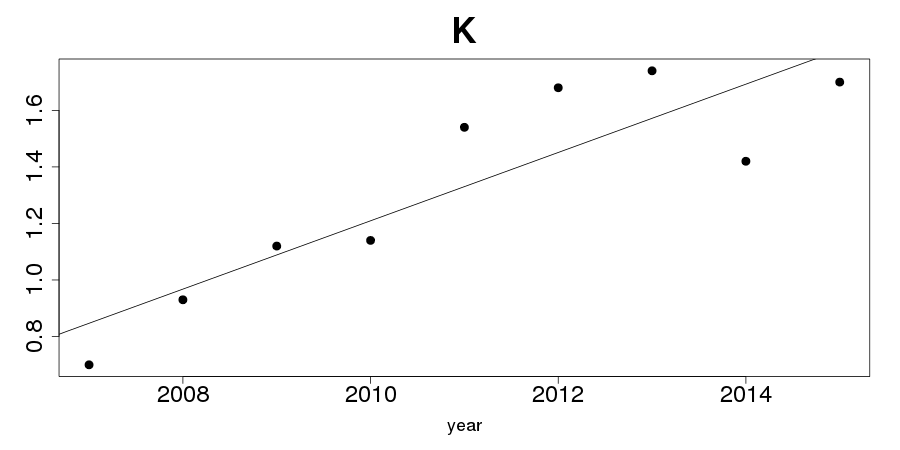
\includegraphics[width=\linewidth]{K}
\caption{{\footnotesize The ratio of the normal places obtained during a season to the number of observational nights}}
\label{fig:K}
\end{wrapfigure}

 Thus the satellites appear in the CCD frame at sufficient distance from the planet. So their coordinates could be mesaured.\par
Let's show this effect by calculating the K coefficient. The K is a ratio of the normal places obtained during an observational season to the number of nights in this season when a series of frames with Uranus was made. The observational season is meant as the period since the end of August to the beginning of January. January observation nights are attributed to previous year. Figure (\ref{fig:K}) illustrates the increase in this ratio.\par


Obtained coordinates were compared with coordinates predicted with the planet motion theory INPOP13c and the theory of uranian satellite motion Lainey 2015. The ephemeris were provided by the MULTI-SAT servise (Emelyanov and Arlot, 2008). Also positions of Uranus were determined based on the positions of its satellites and ephemeris distanses between them and the planet.  The series of the O-C differences for each satellite and for the planet are shown on plots, the average O-C differences are in Table \ref{mean_OC}.
 Observations show a good consent with theory.\par
\begin{table}
\begin{center}
\caption{The average O-C differences}
\label{mean_OC}
\begin{tabular}{|c|c|c|c|c|c|}
\hline
& Ariel&Umbriel&Titania& Oberon & Uranus \\
\hline
Average $(O-C)_\alpha$ & 0.043 & 0.025 & -0.009 & -0.001 & 0.001\\
Average $(O-C)_\delta$ & -0.074 & -0.069 & -0.014 & -0.019 & -0.021\\
\hline
\end{tabular}
\end{center}
\end{table}

\newpage


\begin{figure}[h!]
\begin{minipage}[h]{0.49\linewidth}
\centering{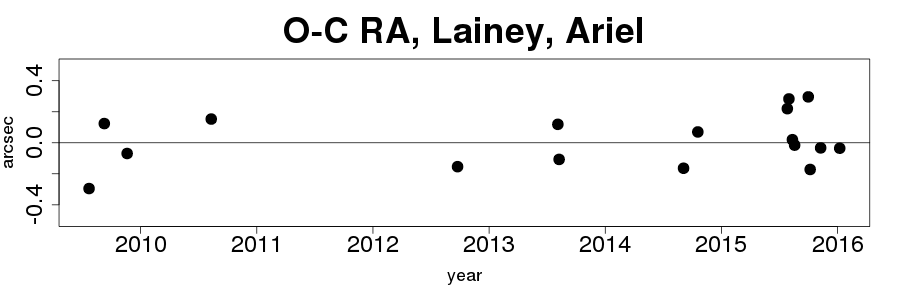
\includegraphics[width=1.0\linewidth]{Ariel_Lainey_RA}\\Ariel, $(O-C)_\alpha$}
\end{minipage}
\begin{minipage}[h]{0.49\linewidth}
\centering{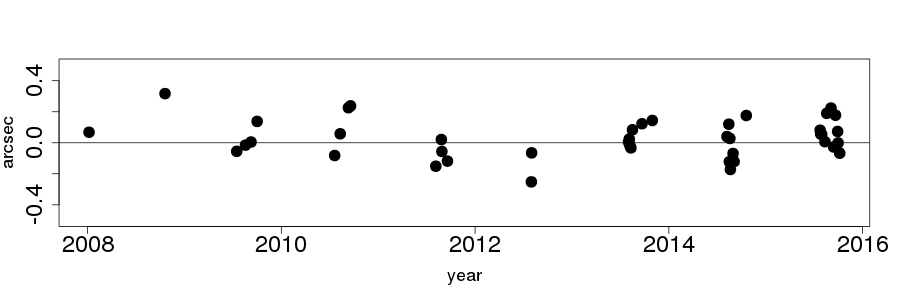
\includegraphics[width=1.0\linewidth]{Umbriel_Lainey_RA}\\Umbriel, $(O-C)_\alpha$}
\end{minipage}
\end{figure}
\begin{figure}[h!]
\begin{minipage}[h]{0.49\linewidth}
\centering{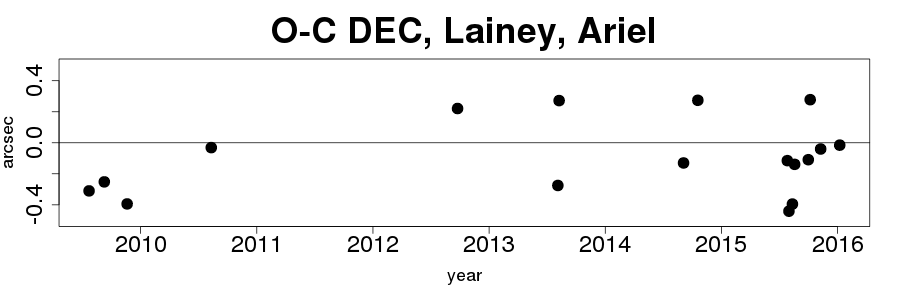
\includegraphics[width=1.0\linewidth]{Ariel_Lainey_DEC}\\Ariel, $(O-C)_\delta$}
\end{minipage}
\begin{minipage}[h]{0.49\linewidth}
\centering{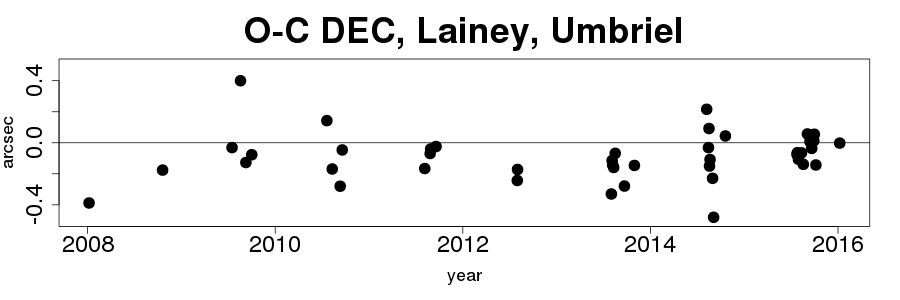
\includegraphics[width=1.0\linewidth]{Umbriel_Lainey_DEC}\\Umbriel, $(O-C)_\delta$}
\end{minipage}
\end{figure}


\begin{figure}[h!]
\begin{minipage}[h]{0.49\linewidth}
\centering{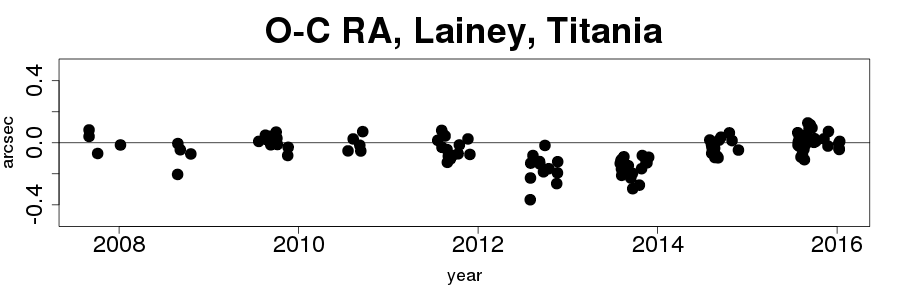
\includegraphics[width=1.0\linewidth]{Titania_Lainey_RA}\\Titania, $(O-C)_\alpha$}
\end{minipage}
\begin{minipage}[h]{0.49\linewidth}
\centering{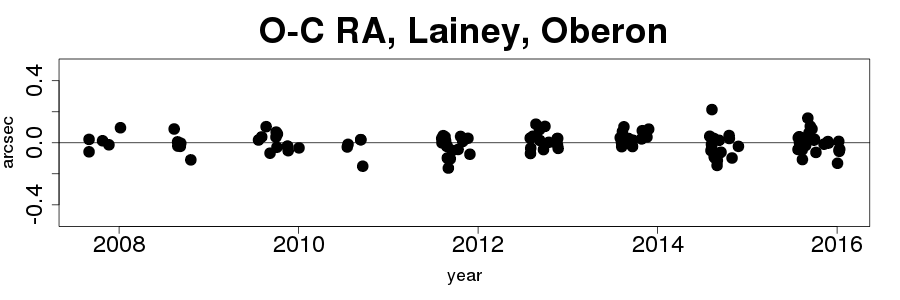
\includegraphics[width=1.0\linewidth]{Oberon_Lainey_RA}\\Oberon, $(O-C)_\alpha$}
\end{minipage}
\end{figure}
\begin{figure}[h!]
\begin{minipage}[h]{0.49\linewidth}
\centering{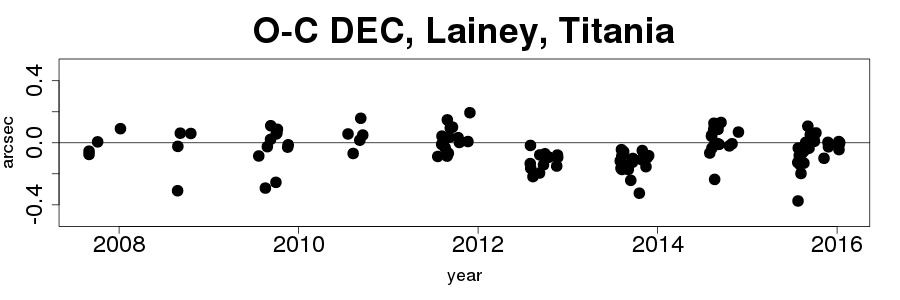
\includegraphics[width=1.0\linewidth]{Titania_Lainey_DEC}\\Titania, $(O-C)_\delta$}
\end{minipage}
\begin{minipage}[h]{0.49\linewidth}
\centering{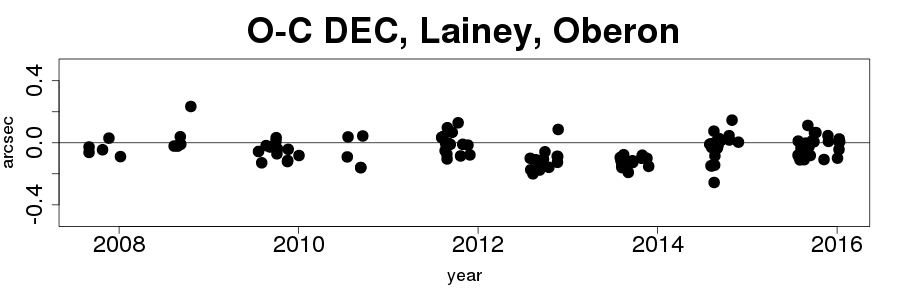
\includegraphics[width=1.0\linewidth]{Oberon_Lainey_DEC}\\Oberon, $(O-C)_\delta$}
\end{minipage}
\end{figure}


\begin{figure}[h!]
\begin{minipage}[h]{0.49\linewidth}
\centering{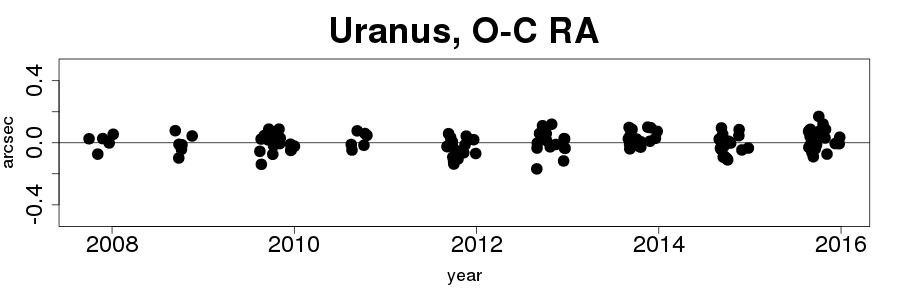
\includegraphics[width=1.0\linewidth]{Uranus_oc_ra}\\Titania, $(O-C)_\alpha$}
\end{minipage}
\begin{minipage}[h]{0.49\linewidth}
\centering{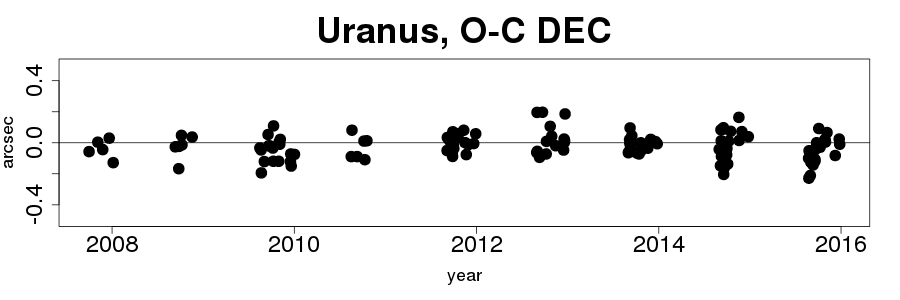
\includegraphics[width=1.0\linewidth]{Uranus_oc_de}\\Oberon, $(O-C)_\alpha$}
\end{minipage}
\end{figure}



\section{Conclusion}
This paper reports the results of observations of the uranian satellites performed in Pulkovo Observatory with the 26-inch refractor in 2007 -- 2016. Result analysis demonstrates high-quality and the suitability of the methods realised in this work, in particular the method of planet halo subtracting. These methods can be applied in the future works on close subjects. Observed positions of the main uranian satellites are usually close to ephemeris position. The obtained normal places are avaliable in the pulkovo database and in the CDS database.

\section{Acknowledgments}





\begin{thebibliography}{99}
\bibitem{1} \textquotedblleft Astrometric Observations of Satellites of Uranus Using 26-Inch Refractor in 2007--2011\textquotedblright, 2013, E. A. Roschina, I. S. Izmailov, T. P. Kiseleva
\bibitem{2}  \textquotedblleft Astrometry of the main satellites of Uranus: 18 years of observations\textquotedblright, 2015, J.I.B. Camargo, F. P. Magalhaes, R. Vieira-Martins, M. Assafin, F. Braga-Ribas, A. Dias-Oliveira,G. Benedetti-Rossi, A. R. Gomes-Junior, A. H. Andrei and D. N. da Silva Neto
\bibitem{7} M.Yu. Khovrichev, Astrometric observations of the Uranian satellites with the Faulkes telescope North in 2007 September, 2009
\bibitem{6} Izmailov I.S., Kiselev A.A., Kiseleva T.P., and Khrutskaya E.V., Using a CCD-camera in Pulkovo programs of observations of binary and multiple stars and satellites of major planets with the 26-inch refractor . Astron. Lett., 1998, vol. 24, no. 5, pp. 665-672.
\bibitem{3}  Izmccd is a software  packet for processing digital images of celestial objects, 2005, Izmailov, I.S., http://www.izmccd.puldb.ru/
\bibitem{4} \textquotedblleft Precision of the ephemerides of outer planetary satellites\textquotedblright, Planetary and Space Science, 2009, Emelyanov N.V.
\bibitem{5} Emelyanov N.V. and Arlot J.-E., The natural satellites ephemerides facility MULTI-SAT, Astron., Astrophis., 2008, vol. 487, pp. 759-765
\bibitem{8} Kiseleva T.P., Khrutskaya E.V., Pulkovo astrometric observations of bodies of the Solar System from 1898 to 2005: observational database, Solar. Syst. Res., 2007 vol. 41, no. 1, pp. 72-80
\bibitem{9} Zacharias, N.; Finch, C. T.; Girard, T. M.; Henden, A.; Bartlett, J. L.; Monet, D. G.; Zacharias, M. I., The Fourth US Naval Observatory CCD Astrograph Catalog (UCAC4), The Astronomical Journal, Volume 145, Issue 2, article id. 44, 14 pp. (2013)
\bibitem{10} Zacharias N., Finch C., Girard T., Hambly N., WycoffG., Zacharias M.I., Castillo D., Corbin, T., DiVittorio, M.,Dutta,  S.,  Gaume,  R.,  Gauss,  S.,  Germain,  M., Hall,  D.,  Hartkopf,  W.,  Hsu,  D.,  Holdenried,  E., Makarov,  V.,  Martinez,  M.,  Mason,  B.,  Monet,  D., Rafferty, T., Rhodes, A., Siemers, T., Smith, D., Tilleman, T., Urban, S., Wieder, G., Winter, L., and Young, A., The third US Naval Observatory CCD Astrograph Catalog   (UCAC3), Astron.   J.,   2010,   vol.   139,   no.   6, pp. 2184?2199.
\end{thebibliography}






\end{document}
